\documentclass[problem]{mcs}

\begin{pcomments}
\pcomment{MQ_sets_to_membership_no_intro}
\pcomment{concise version of MQ_sets_to_membership by ARM 9/20/11}
\pcomment{variant of CP_proving_basic_set_id}
\end{pcomments}

\pkeywords{
  logic
  set_theory
  identity
  propositional
  chain_of_iff
  difference
}
%(A union B) - (A  - B) = B 
%by proving (P v R) ^ NOT(A ^ NOT(B))

%%%%%%%%%%%%%%%%%%%%%%%%%%%%%%%%%%%%%%%%%%%%%%%%%%%%%%%%%%%%%%%%%%%%%
% Problem starts here
%%%%%%%%%%%%%%%%%%%%%%%%%%%%%%%%%%%%%%%%%%%%%%%%%%%%%%%%%%%%%%%%%%%%%

\begin{problem}
Figure \ref{fig:img} shows the arrow diagram for a relation, $R$.

\begin{figure}[h]

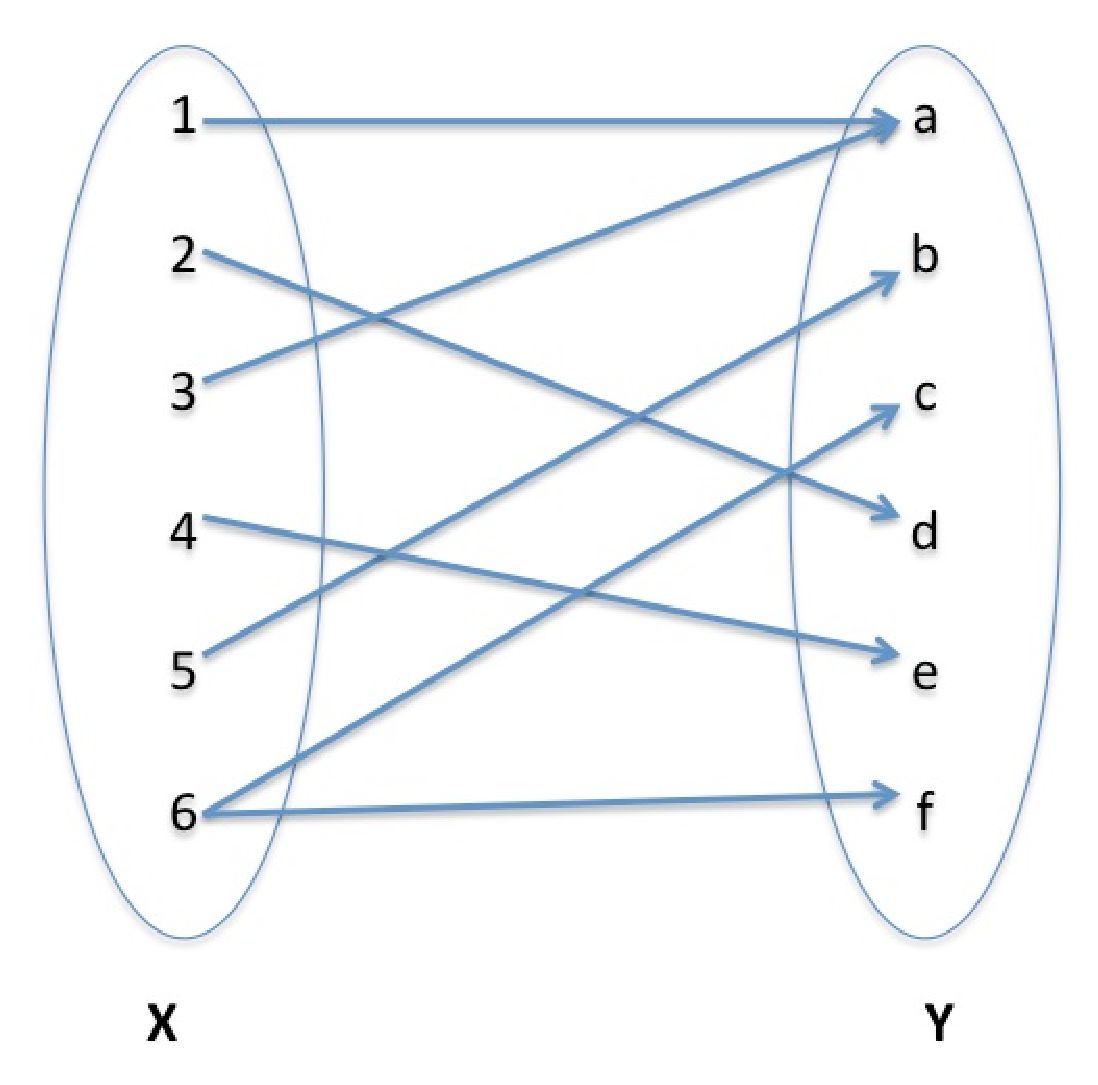
\includegraphics[height = 2in ]{image-inverseimage1}

\caption{Relation $R$.}
\label{fig:img}
\end{figure}
\bparts

\ppart What is the image under $R$ of the even numbers in domain $X$?\hfill\brule{1.5in}

\ppart What is the inverse image under $R$ of the vowels in codomain $Y$?\hfill\brule{1.5in}

\ppart List the first letters of \emph{all} the properties below
satisfied by relation $R$.\hfill\brule{1.0in}
\begin{center}
 \textbf{f}unction \qquad \textbf{t}otal 

 \textbf{i}njective \qquad \textbf{s}urjective
 \qquad \textbf{b}ijective
\end{center}

\eparts

\begin{solution}

\phantom{lol \\}
\phantom{lol \\}
(a) \{d, e, f\}

(b) \{1, 3, 4\}

(c) total ($>= 1$ arrow out) and surjective ($>= 1$ arrow in)

\end{solution}

\end{problem}
%%%%%%%%%%%%%%%%%%%%%%%%%%%%%%%%%%%%%%%%%%%%%%%%%%%%%%%%%%%%%%%%%%%%%
% Problem ends here
%%%%%%%%%%%%%%%%%%%%%%%%%%%%%%%%%%%%%%%%%%%%%%%%%%%%%%%%%%%%%%%%%%%%%

\endinput
